\chapter{Creación de extensiones Chrome a partir del modelo de aumentación}
\label{cha:generador}
\chaptermark{Transformador de extensiones}

En este capítulo se tratan diferentes temas relacionados con la generación de la aumentación para implantarla en el navegador.

Para ubicarse, en primer lugar se realiza una aumentación web con el editor WebMakeUp. Posteriormente, se genera una extensión de Google Chrome. Esta se instala y se ejecuta en el sitio web que se indique en tiempo de edición para mostrar la aumentación que se desea.

Por lo tanto, este capítulo va dedicado a explicar cómo se crea la extensión de Google Chrome a partir del modelo de datos que proporciona en tiempo de edición la herramienta WebMakeUp. En primer lugar, se habla del modelo de aumentación del editor, que es independiente de la plataforma en la que se va a generar (Platform Independent Model, a partir de ahora PIM) en el Apartado \ref{sec:PIM}.

Posteriormente, hay que hablar del modelo específico de dominio (Platform Specific Model, a partir de ahora PSM), donde en este PFG se decide crear una extensión de Google Chrome utilizando como base algunas librerías entre la que se destaca ConstraintJS. Para ello, hay que explicar claramente cómo es la plataforma y cómo es el modelo resultante de la transformación.

Asimismo, hay que describir cómo se hace esa transformación y cómo se ejecuta la aumentación (Apartado \ref{sec:DescripcionGenerador}).

Finalmente se muestran algunos ejemplos de aumentación (Apartado \ref{sec:EjemplosGenerador}) y una validación final en base a los patrones y tipos de widgets existentes (Apartado \ref{sec:ValidacionGenerador}).

\section{Platform Independent Model - Modelo independiente de la plataforma}
\label{sec:PIM}

A la hora de crear una extensión, en primer lugar hay que explicar cuál es el proceso. En el editor WebMakeUp, la aumentación se refleja de manera gráfica para el usuario. Además existe un modelo asociado a la aumentación, que es el que se encarga de representarla internamente.

Esta representación interna puede servir para 2 aspectos en prácticamente cualquier editor del mercado:
\begin{itemize}
\item{Permitir dar persistencia en el trabajo que se está realizando, lo que habitualmente se denomina guardar. Asociado con el concepto de guardar un proyecto del editor, existe la opción inversa, que es cargar un proyecto en el editor. Para permitir esto, hay que representar en un modelo de datos el trabajo que se está realizando.}
\item{Permitir exportar los resultados del trabajo, generando un resultado, que al final es el que se va a utilizar. Para ello también se utiliza un modelo de datos.}
\end{itemize}

Este PFG se ha centrado en una pequeña parte de exportar un resultado final, todo ello a partir del modelo de datos que proporciona WebMakeUp. El trabajo realizado es el empaquetamiento de la extensión y el modelo de interacción (ver Capítulo \ref{cha:interacciones}). Asimismo, en WebMakeUp pero fuera del PFG se trabaja con la creación en tiempo de ejecución de los widgets y el posicionamiento del mismo. Sobre esto último también hay que comentar algunos aspectos, dado que pertenece todo al transformador.

En la Figura \ref{fig:MetamodeloWebMakeUp} se muestra todo el metamodelo de WebMakeUp. En el se representan todos los aspectos de la aumentación: propiedades de los widgets (la clase Widget y sus relaciones), propiedades de interacción (representado mediante Blinks), y de la propia aumentación (la clase Mod).

\begin{figure}
\begin{center}
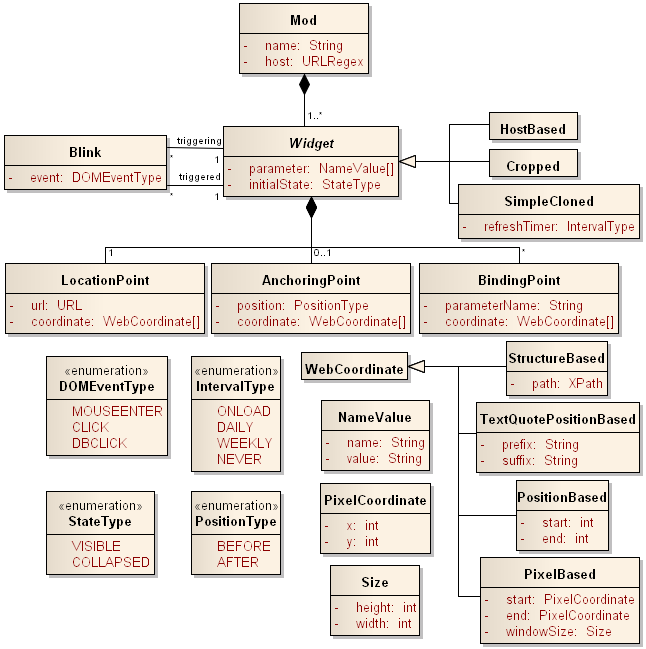
\includegraphics[width=0.65\textwidth]{figs/5-MetamodeloWebMakeUp.png}
\caption{Metamodelo de WebMakeUp que representa cómo es una aumentación web.}
\label{fig:MetamodeloWebMakeUp}
\end{center}
\end{figure}

Este PFG se centra únicamente en las clases del metamodelo que representan las configuraciones de la extensión (la clase \textbf{Mod}) y en cómo generar un código que sea capaz de plasmar las interacciones (la relación entre \textbf{Widgets} mediante \textbf{Blinks}). Estas clases del metamodelo se pueden ver en la Figura \ref{fig:MetamodeloWebMakeUpReducido}. 

Asimismo, hay widgets que acceden a recursos fuera del sitio web donde se ejecuta la aumentación. Esto requiere de permisos adicionales, dado que por defecto una aumentación sólo puede acceder al sitio web donde se ejecuta. Por lo tanto, la clase \textbf{LocationPoint} almacena las URLs externas a las que tiene acceso un Widget. Con ello se consigue en tiempo de transformación indicar a la extensión de Google Chrome los permisos estrictamente necesarios, ofreciendo mayor seguridad a las aumentaciones creadas.

\begin{figure}
\begin{center}
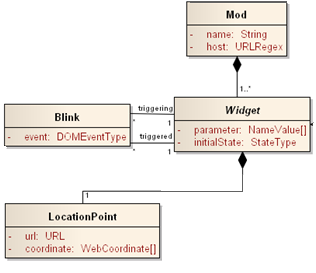
\includegraphics[width=0.45\textwidth]{figs/5-MetamodeloWebMakeUpReducido.png}
\caption{Parte del metamodelo de WebMakeUp del que se extrae la información de la aumentación y las animaciones.}
\label{fig:MetamodeloWebMakeUpReducido}
\end{center}
\end{figure}


\section{Platform Specific Model - Modelo especifico de la plataforma}
\label{sec:PSM}

En este apartado se trata de definir cómo es la plataforma sobre la que va a ejecutarse la aumentación. Es necesario conocer cómo es la plataforma para poder generar un artefacto acorde a las especificaciones que se detallan en la propia plataforma.

Cómo se ha ido comentando a lo largo de este documento, la plataforma sobre la que se ha trabajado ha sido Google Chrome. WebMakeUp está desarrollado sobre Google Chrome y las aumentaciones que crea son específicamente para Google Chrome. Por tanto, se debe hablar de cómo es Google Chrome (Apartado \ref{sec:PSM-GoogleChrome}).

\subsection{Google Chrome}
\label{sec:PSM-GoogleChrome}
Google Chrome es un navegador Web de uso general. El navegador ha sido desarrollado a partir del proyecto Chromium\footnote{Web del proyecto Chromium: \url{http://www.chromium.org/}}, pero el navegador que este proyecto ofrece no está apoyado ni comercial ni técnicamente por Google.

En este PFG, el uso de Google Chrome fue impuesto, por tanto no se tuvo que realizar ningún tipo de estudio sobre qué plataforma utilizar para el desarrollo de WebMakeUp, ni tampoco de las aumentaciones que se crean. Aun así, es necesario mencionar el porqué Google Chrome en lugar de otros. 

Existe una razón principal, que es el uso de Google Chrome en el mercado. Google Chrome se lanza al mercado de manera oficial en septiembre de 2008. Como se muestra en la Figura \ref{fig:UsoGoogleChrome} a mediados de 2012 ya consigue desbancar a Internet Explorer como navegador más utilizado. Actualmente presenta una cuota de un 45\% de uso en el mercado, tanto en PC, como en otros dispositivos.

\begin{figure}
\begin{center}
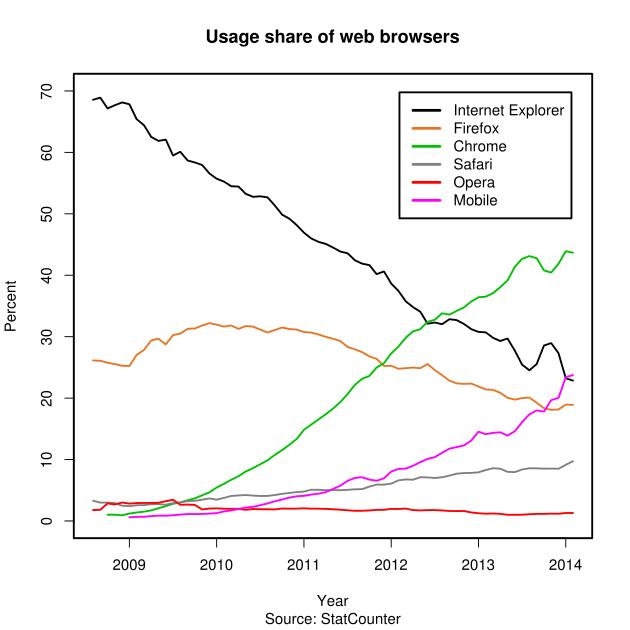
\includegraphics[width=0.65\textwidth]{figs/5-UsoGoogleChrome.png}
\caption{Utilización de Google Chrome en el mercado.}
\label{fig:UsoGoogleChrome}
\end{center}
\end{figure}

En este caso, únicamente hay que comentar cómo es Google Chrome para PC, ya sea en sus versiones para Windows, MacOS o Linux, que presentan una interfaz prácticamente idéntica (no únicamente gráfica, sino también de desarrollo).

Google Chrome, al igual que otros navegadores actuales ofrecen posibilidades de extensión de las funcionalidades que ofrecen. Esta extensibilidad del navegador en Google Chrome se pueden hacer de 2 formas. Por un lado existen las \emph{apps} y por otro lado las extensiones.

Las Google Chrome apps\footnote{Google Chrome apps:\url{https://support.google.com/chrome/answer/1050586?hl=en}} en realidad son aplicaciones puramente del lado servidor. Google Chrome permite la instalación de estas apps y con ello tener un acceso directo desde el navegador o incluso desde el propio sistema operativo.

En este caso al trabajar con aumentación web esta opción no es interesante, dado que se requiere de un lado servidor del que no se va a disponer. Por tanto, existen las extensiones, que permiten modificar las funcionalidades y tareas que realiza el navegador de manera local. Es decir, la extensión se ejecuta en el lado cliente y no repercute en el lado servidor.

Existen 2 maneras de desarrollar extensiones en Google Chrome, mediante el uso de \emph{userscripts} o mediante extensiones nativas de Google Chrome.

Un \emph{userscript}\footnote{Ejemplos de userscript:  \url{http://userscripts.org:8080/}} está constituido por un fichero, que es un \emph{script}, programado en Javascript. Este brinda la posibilidad de hacer modificaciones en el DOM del sitio web y aplicar algunas cláusulas de permisos, y de recursos utilizados. Estos \emph{userscript} pueden ser utilizados en cualquier navegador que sea capaz de interpretarlos. Actualmente tanto Firefox como Google Chrome son capaces de interpretarlos de manera nativa.

Inspirado en los \emph{userscript}, Google Chrome dispone de extensiones nativas. Con inspirado se quiere decir que el creador de los \emph{userscript}, también participó en el desarrollo de la extensiones de Google Chrome y que la especificación de algunas cosas son similares. La principal diferencia es que una extensión de Google Chrome permite no solo el acceso al DOM, si no a múltiples características del propio navegador (como la persistencia de datos). En el caso del editor de mods WebMakeUp, se pueden almacenar aumentaciones sin exportar y recuperarlas para seguir editando en otro momento. Para ello utiliza la persistencia que ofrece Google Chrome en su API\footnote{Persistencia en Google Chrome mediante HTML5 y javascript: \url{http://mysticalpotato.wordpress.com/2011/01/23/html5-y-json-para-dotar-de-persistencia-a-una-extension-de-chrome/}}.

Las extensiones nativas de Google Chrome se pueden instalar de 2 maneras.

Por un lado, existe el Chrome Store\footnote{Sitio web del Chrome Store: \url{https://chrome.google.com/webstore}}, que es una tienda online que permite instalar apps y extensiones nativas en un clic, mantiene la sincronización entre los diferentes PCs con Chrome donde se tenga la cuenta de Google iniciada. El fichero que se instala es un contenedor firmado por el creador de la extensión y que garantiza la integridad del mismo ofreciendo seguridad.

Por otro lado, existe la posibilidad de instalarla desde el PC, desde una carpeta que cumpla con las especificaciones de una extensión de Google Chrome que se explica a continuación. Dado que en este PFG no se abarca la posibilidad de publicación de la extensión que el usuario crea con el editor WebMakeUp, lo que se crea es un comprimido .zip con el código necesario para implantar y ejecutar la aumentación en el navegador.

Las extensiones de Google Chrome son sencillas de programar. Para ello Google Chrome interpreta los 3 lenguajes del lado cliente que se utilizan en el desarrollo del lado cliente de la web, HTML, CSS y Javascript. En las extensiones nativas, al igual que en los \emph{userscripts} predomina Javascript, dado que el contenido de la web ya existe (se obtiene de un sitio web). Muchas veces los estilos también se mantienen dado que las extensiones habitualmente cambian la funcionalidad y pocas veces en el estilo. Por tanto, los mayores cambios se van a notar en el comportamiento del sitio y eso corresponde a Javascript.

En Google Chrome existen diferentes áreas de trabajo. La estructura de una extensión divide las zonas de acción de la extensión. Tal y cómo se muestra en la Figura \ref{fig:arquitecturaChrome}, existe un fichero principal, llamado \emph{manifest.json}.

\begin{figure}
\begin{center}
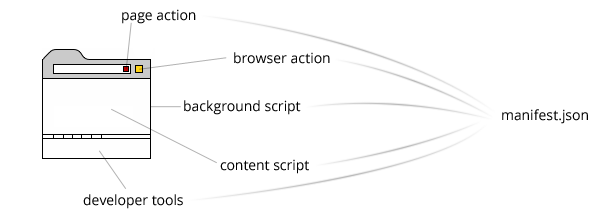
\includegraphics[width=0.75\textwidth]{figs/5-chromeArchitecture.png}
\caption{Arquitectura de desarrollo de Google Chrome donde se observa en qué parte actúa cada área de la extensión.}
\label{fig:arquitecturaChrome}
\end{center}
\end{figure}

El manifest.json es el único fichero en una extensión de Google Chrome que es obligatorio. En la Figura \ref{fig:chromeManifest} se observa un fichero básico manifest.json que ayudará a explicar la estructura que se necesita para desarrollar una extensión.

\begin{figure}
\begin{center}
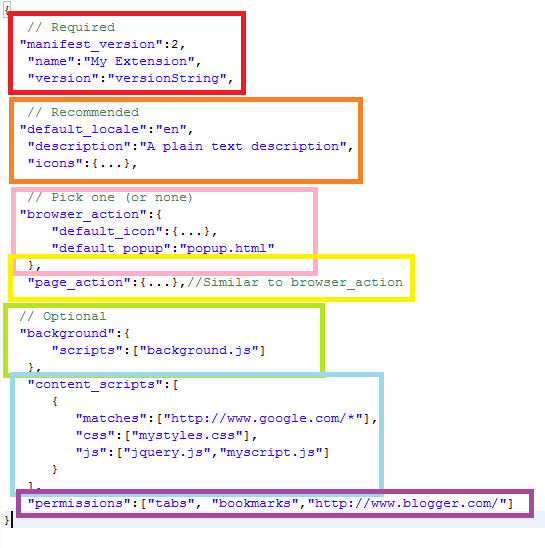
\includegraphics[width=0.65\textwidth]{figs/5-Manifest.png}
\caption{Estructura básica del fichero de manifest.}
\label{fig:chromeManifest}
\end{center}
\end{figure}

Por un lado, se gestionan las propiedades generales (en negrita se marcan las obligatorias):
\begin{itemize}
\item{\textbf{Versión del manifiesto}: actualmente se utiliza la v2. En los \emph{userscript}, que también tienen su propio manifiesto, se utilizaba la v1, aunque ya está obsoleta.}
\item{\textbf{Nombre}: nombre de la extensión.}
\item{\textbf{Versión}: versión en la que se encuentra la extensión creada.}
\item{Descripción: descripción de la extensión. Se suele utilizar para describir para qué sirve la extensión o dónde se utiliza.}
\item{Permisos: a qué recursos puede acceder la extensión. Qué sitios web, si utiliza persistencia para almacenar los datos, etc.}
\end{itemize}

Por otro lado, se definen los ficheros que conforman las diferentes áreas de trabajo que se muestran en la Figura \ref{fig:arquitecturaChrome}:
\begin{itemize}
\item{Page action: su uso común es el de notificar dentro de la barra de dirección/búsqueda de Chrome.}
\item{Browser action: proporciona un menú para la extensión. Por ejemplo en WebMakeUp ahí está el menú para iniciar el editor, guardar, cargar y exportar la aumentación.}
\item{Background script: cada extensión crea un nuevo proceso de Google Chrome en el sistema operativo. Cada pestaña también tiene su propio proceso. El background es código que se ejecuta en el proceso de la extensión y lo comparten todas las pestañas. Dispone de algunos permisos cómo acceso a componentes del navegador, por ejemplo, para poder almacenar datos.}
\item{Content script: lo conforman los scripts que se ejecutan en una pestaña concreta. Se le pueden indicar en qué sitios webs tiene que actuar. En la Figura \ref{fig:chromeManifest} de color azul se observa en matches que actuará solo en el sitio de \url{www.google.com} y que se interpretarán dos Javascripts y un fichero de CSS. Dispone de acceso al DOM, pero no puede acceder a componentes del navegador.}
\end{itemize}

Una aumentación el único fin que tiene es modificar el DOM, que es donde se trabaja con los widgets que están dispuestos en él. Por tanto, lo razonable es que la aumentación que se va a generar trabaje sobre el content script.

En el Apartado \ref{sec:DescripcionGenerador} se habla sobre como funciona el transformador de la extensión en base al modelo de datos que proporciona WebMakeUp (Apartado \ref{sec:PIM}) y junto a la plataforma especifica (Google Chrome) que se ha descrito en este apartado.

\section{Descripción de la transformación de la extensión}
\label{sec:DescripcionGenerador}

Antes de comenzar a explicar cómo se obtiene la transformación de la extensión, hay que tener claro un concepto relacionado con Javascript. Tal y como se ha ido mencionando en apartados anteriores, Javascript es un lenguaje interpretado.

El lenguaje de programación C es un lenguaje que se compila obteniendo un código ejecutable por la máquina. Este código, posteriormente se ejecuta en una máquina que cumpla con las mismas características (como la arquitectura de la CPU).

En Javascript, el código fuente no se compila. Existe un intérprete (llamado motor Javascript) que es capaz en tiempo de ejecución de interpretar ese código y ejecutarlo. Cada navegador tiene su propio intérprete y no todos interpretan las instrucciones de la misma manera. Para ello, existen estándares como \emph{ECMAScript} que permiten garantizar que esa interpretación será idéntica en los diferentes intérpretes existentes en el mercado.

¿Qué ventajas ofrece que sea interpretado? Permite que el mismo fichero .js sea multiplataforma. Esto es lógico hacerlo dado que Javascript es un lenguaje de uso en Internet, donde los usuarios disponen de diferentes plataformas y acceden al mismo contenido.

Una vez aclarado cómo funciona Javascript, hay que dividir la transformación de la extensión en dos fases. Por un lado, la generación/creación de la extensión de Google Chrome, y por otro lado, la ejecución de la misma.

\subsection{Creación de la extensión de Chrome}
\label{sec:CreacionExtension}

En este apartado el objetivo es sencillo. Hay que realizar una traducción del lenguaje que conoce WebMakeUp (el modelo de datos de la aumentación) al lenguaje que conoce Google Chrome (la arquitectura de extensión nativa de Google Chrome).

Dado que se ha decidido interpretar el modelo en tiempo de ejecución (ver Apartado \ref{sec:EjecucionExtension}), en la creación de la extensión simplemente hay que generar el manifest.json y el modelo de datos que posteriormente se interpreta.

El manifest.json tiene una parte que es común a todas las extensiones que se generan y una parte dinámica dependiendo de la aumentación. En la Figura \ref{fig:generatedManifestStaticDynamic} se diferencian los campos comunes a todas las extensiones (versión, estilos y Javascripts a ejecutar en el context script), y las variables dependiendo de la aumentación que se cree (nombre, descripción, sitios webs donde se ejecuta y permisos).

\begin{figure}
\begin{center}
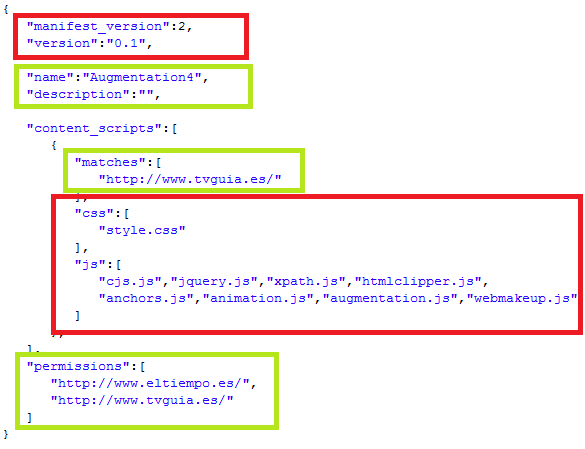
\includegraphics[width=0.65\textwidth]{figs/5-generatedManifestStaticDynamic.png}
\caption{Fichero manifest.json donde se diferencia la parte común (rojo) a todas las extensiones de la parte variable (verde).}
\label{fig:generatedManifestStaticDynamic}
\end{center}
\end{figure}

Estos datos se obtienen del modelo, en este caso de las clases que se presentan en la Figura \ref{fig:MetamodelReducedManifest}.

\begin{figure}
\centering
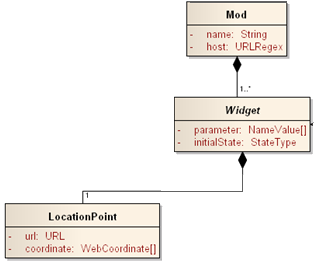
\includegraphics[width=0.5\textwidth]{./figs/5-MetamodelReducedManifest}
\caption{Parte del metamodelo que se utiliza en tiempo de generación de la extensión.}
\label{fig:MetamodelReducedManifest}
\end{figure}


Un \emph{Mod} tiene un nombre, una descripción y una \emph{URLRegex}, que es una expresión regular que indica el sitio/sitios donde se va a ejecutar.

A su vez, dependiendo de los widgets, estos pueden ser de diferentes tipos. Si estos requieren obtener algún tipo de datos de otro sitio web se tiene que proporcionar permisos para ello. Cada widget dispone de un location point con la URL a la que accede y en este caso lo que se hace es añadirla a los sitios permitidos.

Además del manifest, hay que importar el modelo de WebMakeUp para que se interprete en tiempo de ejecución. Para ello se realiza una conversión del objeto JSON que contiene todo el modelo de datos de WebMakeUp a \emph{string} gracias a la función \emph{JSON.stringify()} de Javascript.

Finalmente, se empaquetan todas las librerías necesarias para su futura interpretación en \emph{runtime} (tiempo de ejecución), para presentarle al usuario un fichero .zip comprimido con la extensión generada. Para empaquetar la extensión se utiliza una librería llamada JSzip \footnote{Web oficial de jszip: \url{http://stuk.github.io/jszip/}}. En ella se convierten los \emph{strings} en ficheros incluidos en un objeto \emph{BLOB} (Objeto Binario Largo) que actúa de contenedor. Para presentarle este objeto al usuario, se ha utilizado la librería FileSaver\footnote{Sitio web oficial de FileSaver: \url{https://github.com/eligrey/FileSaver.js/}}. Con ella se hace una descarga del BLOB, que en este caso es un fichero contenedor en .zip.

El resultado final es el que se presenta en la Figura \ref{fig:ExtensionEmpaquetada}. En él se incluye el fichero manifest.json que se ha generado y el fichero webmakeup.js que incluye el modelo de datos en formato JSON. El resto de ficheros sirven para interpretar el modelo y poder ejecutar la aumentación en \emph{runtime}.

\begin{figure}
\centering
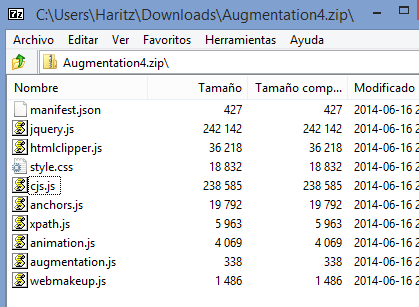
\includegraphics[width=0.7\linewidth]{./figs/5-ExtensionEmpaquetada}
\caption{Extensión empaquetada que se genera a partir de la aumentación}
\label{fig:ExtensionEmpaquetada}
\end{figure}


\subsection{Ejecución de la extensión}
\label{sec:EjecucionExtension}

Una vez generada la extensión (Apartado \ref{sec:CreacionExtension}), en este apartado se habla de cómo se interpreta el modelo de datos para crear la aumentación.

Tal y como se ha comentado previamente, el código puede ser compilado o interpretado. Incluso en el propio WebMakeUp en tiempo de generación se puede haber compilado (o creado) las instrucciones Javascript que se van a ejecutar. Como prueba de ello, en la primera versión de WebMakeUp basada en diagramas de transición de estados se generaban las instrucciones Javascript. En la Figura \ref{fig:generatedCompiledCodeSTD} se muestra que los datos están en el propio código. Se reflejan los estados que se crean y las transiciones existentes, donde los parámetros de las funciones a las que se llaman están estos datos sin ofrecer ninguna estructura.

\begin{figure}
\centering
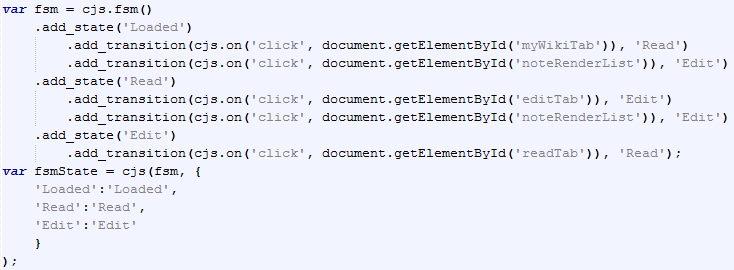
\includegraphics[width=0.95\linewidth]{./figs/5-generatedCompiledCodeSTD}
\caption{Código pre-compilado con la máquina de transición de estados que se crea en tiempo de ejecución.}
\label{fig:generatedCompiledCodeSTD}
\end{figure}

El realizarlo de esta manera no supone ninguna ventaja práctica, dado que la ventaja principal del código compilado es que se ejecuta más rápido, pero Javascript es interpretado. Por tanto interpretar un código que interpreta un modelo de datos en coste es prácticamente idéntico a un código con las funciones a ejecutar ya preparadas para ser interpretadas.

Las ventajas de generar únicamente un modelo e interpretarlo en tiempo de ejecución, sin embargo, son notorias:
\begin{itemize}
\item{Es más fácil de validar un modelo de datos que la sintaxis y semántica de un lenguaje de programación. Existen herramientas como JSON Schema con el que se pueden validar modelos de datos en JSON, además su coste es pequeño.}
\item{Permite evitar dependencia entre datos y código a ejecutar. Por ejemplo, se puede mantener el mismo modelo de datos y cambiar únicamente el intérprete del modelo. Modificarlo es sencillo, mientras que cambiar el generador de instrucciones Javascript es complejo.}
\item{Es más sencillo hacer re-ingeniería. Al estar independizada la parte del modelo de la interpretación es más sencillo reestructurar los procesos, realizar refactorización, etc.}
\end{itemize}

Tras aclarar el porqué se ha realizado un código que interpreta un modelo, sólo queda por describir cómo se interpreta.

Cabe destacar que del modelo hay que interpretar tanto los widgets como las animaciones. El intérprete de widgets no es parte del PFG, por tanto, simplemente hay que mencionar que su objetivo es crear y posicionar los widgets en el DOM. El intérprete de animaciones si es parte del PFG y es en el que se centra este apartado.

\begin{figure}
\centering
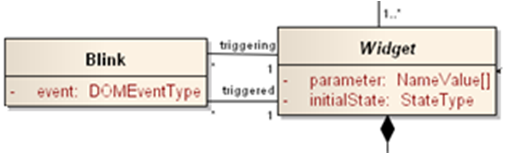
\includegraphics[width=0.7\linewidth]{./figs/5-MetamodelReducedWidgetsBlinks}
\caption{Modelo de datos que describe los blinks de interacción entre widgets}
\label{fig:MetamodelReducedWidgetsBlinks}
\end{figure}

En la Figura \ref{fig:MetamodelReducedWidgetsBlinks} se observan las clases del metamodelo que describen las interacciones basadas en blinks. Como se describe en el Apartado \ref{sec:modeloBlinks}, el blink consta de 2 widgets, un observador (\emph{triggered}) y un controlador (\emph{triggering}), y de un evento que se produce en el \emph{triggering}.

La idea que se ha tenido para representar estas interacciones ha sido mediante STD (diagramas de transición de estados), que en lo que a código se traducen como máquinas de estado finitas (a partir de ahora FSM). Existen dos razones principales para ello:
\begin{itemize}
\item{La previa utilización de FSMs para trabajar con el concepto de estado global de la aumentación en el modelo de interacción basado en STD (Apartado \ref{sec:modeloSTD}).}
\item{La facilidad de representar el concepto de estado de un widget con la misma herramienta que se representaba el estado global (ConstraintJS, descrito en el Anexo \ref{sec:CJS}). Además, la manera de gestionar los manejadores para los diferentes eventos es muy sencilla.}
\end{itemize}

Teniendo en cuenta esto, lo que se genera es una FSM por cada uno de los widgets que tiene al menos un blink en el que participa como observador (\emph{triggered}). Es lógico, dado que ese widget cambiará de estado (de mostrarse a ocultarse y viceversa). Sobre otros widgets (o sobre sí mismo) se pueden producir eventos. Cada vez que se produce un evento sobre un controlador (\emph{triggering}) el observador cambiará de estado. 

En la Figura \ref{fig:blink2WidgetsExample} se muestra un ejemplo que sirve para explicar el cómo se describen las máquinas de estado. En él se presentan tres widgets. Lo que se busca es focalizarse únicamente en el texto superior. Para ello en caso de que se tenga el cursor en el texto superior (Widget 2) las noticias se ocultan (Widget 3). Pero también se puede ocultar el Widget 3 utilizando el widget central (Widget 1) si se hace clic sobre él.

\begin{figure}
\centering
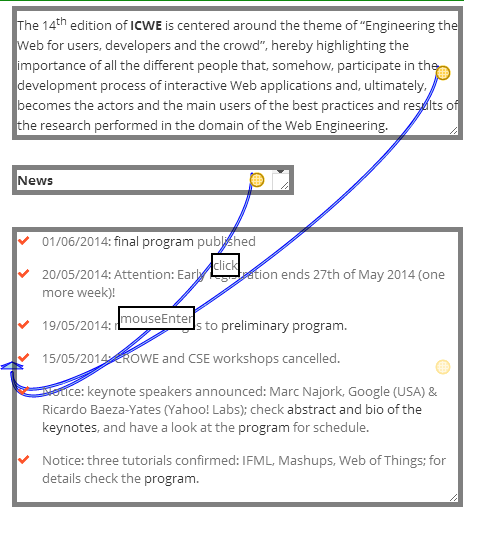
\includegraphics[width=0.5\linewidth]{./figs/5-blink2WidgetsExample}
\caption{Ejemplo de 2 blinks donde el observer es el mismo}
\label{fig:blink2WidgetsExample}
\end{figure}

En la Figura \ref{fig:WidgetFSM} se muestra un cómo se representa en FSM el ejemplo anterior. El widget triggered tiene como estado inicial enable. Existe un blink entre triggered y Widget1 (triggering) con el evento click. Esto significa según el funcionamiento de los blinks, que con el evento click cambia de collapse a enable y con su inverso (el click) vuelve a collapse. Asimismo con el Widget 2 existe un evento que hace que se oculte (mouseover) y otro que con el que vuelve a mostrarse (mouseout).

\begin{figure}
\centering
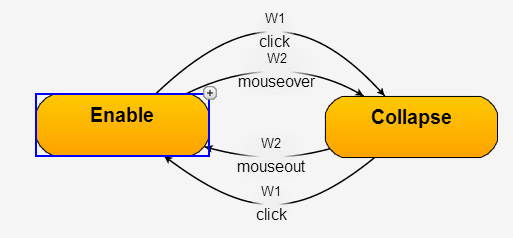
\includegraphics[width=0.7\linewidth]{./figs/5-WidgetFSM}
\caption{Representación en FSM de los estados y transiciones sobre un widget.}
\label{fig:WidgetFSM}
\end{figure}

Por tanto, el intérprete basándose en el modelo de datos debe realizar dos tareas. Por un lado, identificar todos los widgets que participan como triggered en algún blink. Por otro lado, generar para cada uno de esos widgets una FSM con sus eventos y los widgets triggering que participan respectivamente.

Para el primer paso se ha de hacer un recorrido por todos los blinks e ir almacenando por cada widget triggered una lista con los blinks (par evento+triggeringWidget). En la Figura \ref{fig:TriggeredWidgetsJavascript} se puede observar el algoritmo.

\begin{figure}
\centering
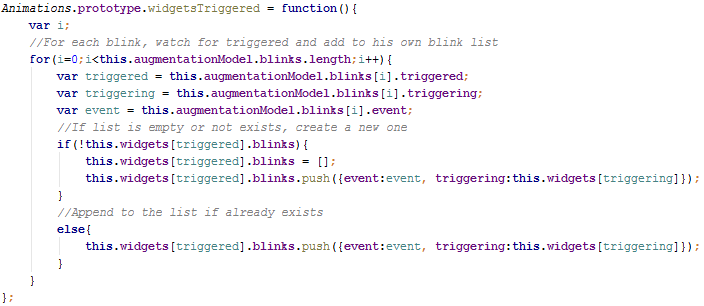
\includegraphics[width=0.7\linewidth]{./figs/5-TriggeredWidgetsJavascript}
\caption{Obtención de los widgets con algún blink en el que tiene la función de observador (triggered).}
\label{fig:TriggeredWidgetsJavascript}
\end{figure}

Para el segundo paso, una vez se obtiene la lista de widgets triggered, utilizando la API de ConstraintJS se crea una FSM para cada widget. La creación como se observa en la Figura \ref{fig:CJSFSMCreation} se realiza en 4 pasos:
\begin{itemize}
\item{Crear los estados de la máquina: enable y collapse.}
\item{Crear un par de transiciones (evento y evento inverso) por cada blink en el que participa como triggered.}
\item{Indicar el estado inicial de la máquina dependiendo del estado inicial del widget.}
\item{Añadir el evento a ejecutar cuando se cambia de estado. De enable->collapse se oculta el widget y de collapse->enable se muestra.}
\end{itemize}

\begin{figure}
\centering
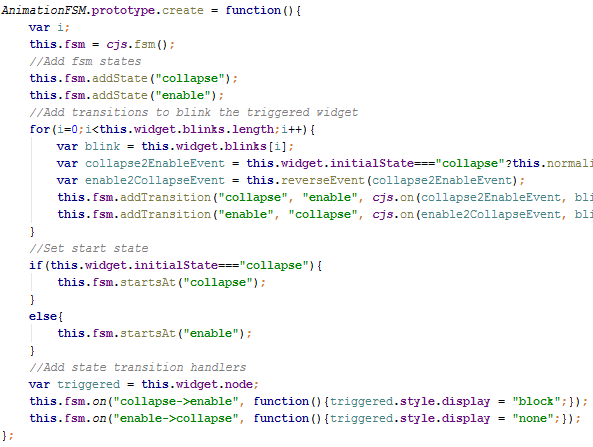
\includegraphics[width=0.7\linewidth]{./figs/5-CJSFSMCreation}
\caption{Creación de la FSM utilizando la API de ConstraintJS}
\label{fig:CJSFSMCreation}
\end{figure}

Una vez creada la FSM, ConstraintJS se encarga de gestionar todos los eventos, las transiciones y los estados de las diferentes máquinas que se crean.

\section{Ejemplos}
\label{sec:EjemplosGenerador}

En este apartado se trata de demostrar el correcto funcionamiento en base a varios ejemplos en diferentes sitios webs y con diferentes tipos de aumentaciones. Estos ejemplos sirven para poder realizar una validación del correcto funcionamiento del transformador (Apartado \ref{sec:ValidacionGenerador}).

El \textbf{ejemplo 1} trata de encaminar los diferentes pasos que hay que realizar para enviar una respuesta a una pregunta en el foro \url{www.stackoverflow.com}. En la Figura \ref{fig:StackOverflowDefault} se observa un formulario en tres pasos. Paso 1, responder la pregunta que se ha hecho. Paso 2, se indican los datos de usuario. Paso 3, se envía la respuesta aceptando los términos de acuerdo. En la Figura \ref{fig:StackOverflowEditor} se muestra que se ha aplicado el patrón zoom-in para ese formulario. Asimismo, abajo hay un widget que muestra un mensaje de si se quiere realizar un tour por StackOverflow. A este widget se le ha aplicado el patrón self-erasable, que una vez leído, si no te interesa el tour se hace clic y elimina el mensaje.

\begin{figure}
\centering
\subfloat[Formulario StackOverflow original]{
	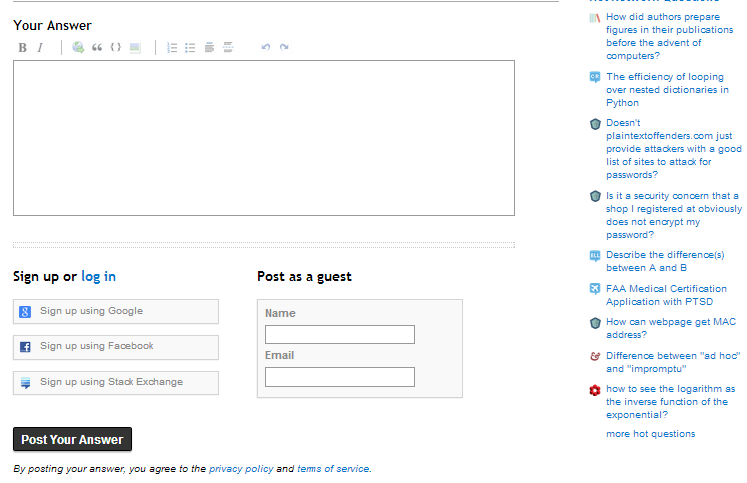
\includegraphics[width=0.5\textwidth]{./figs/5-StackOverflowDefault.png}
	\label{fig:StackOverflowDefault}
}
\subfloat[Editor WebMakeUp aumentando StackOverflow]{
	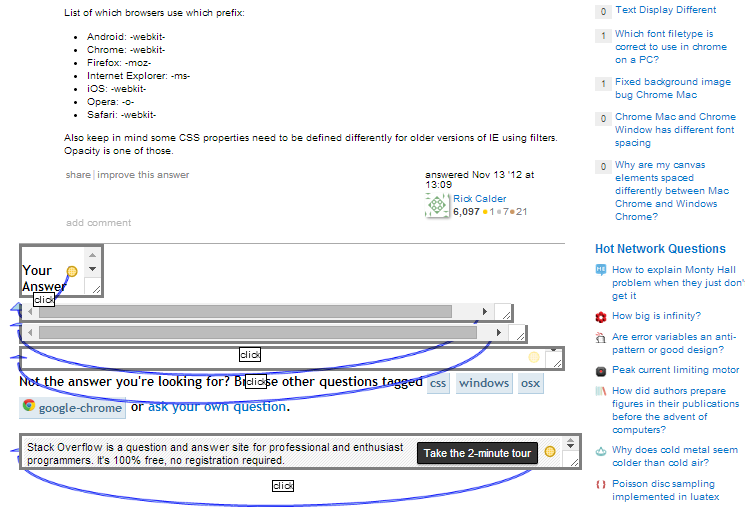
\includegraphics[width=0.5\textwidth]{figs/5-StackOverflow.png}
	\label{fig:StackOverflowEditor}
}
\caption{Ejemplo de aumentación del sitio web StackOverflow.}
\label{fig:StackOverflowExample}
\end{figure}

El \textbf{ejemplo 2} aumenta el sitio \url{http://icwe2013.webengineering.org/program}, que trata sobre el congreso ICWE. En la Figura \ref{fig:ICWEDefault} se muestra en la parte superior izquierda el programa del congreso que se puede o mirar online o descargar. Para aumentarlo, se añade la opción de mostrar u ocultar ambas opciones haciendo clic en el texto Program (Figura \ref{fig:ICWEEditor}). En la inferior izquierda, se muestra el programa para el día 12 de julio. Lo que se ha hecho es utilizando un patrón zoom-in dominó ir mostrando el programa a medida que se va haciendo click en el evento actual, este mostrará el siguiente. Al hacer click en el último evento vuelve a ocultar todos dejándolo compactado. En la parte derecha se ha utilizado un patrón alternate para ir alternando entre los sponsors y los organizadores del ICWE.

\begin{figure}
\centering
\subfloat[Programa del congreso ICWE]{
	
\includegraphics[width=0.5\textwidth]{./figs/5-ICWEDefault.png}
	\label{fig:ICWEDefault}
}
\subfloat[Editor WebMakeUp aumentando ICWE]{
	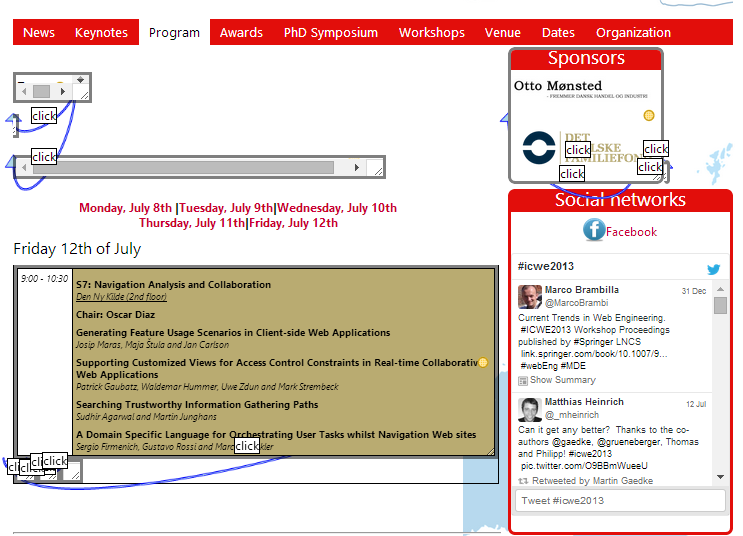
\includegraphics[width=0.5\textwidth]{figs/5-ICWEEditor.png}
	\label{fig:ICWEEditor}
}
\caption{Ejemplo de aumentación del sitio web de ICWE2013.}
\label{fig:ICWEExample}
\end{figure}

En el \textbf{ejemplo 3} se ha aumentado \url{www.tvguia.es} (ver Figura \ref{fig:TVGuiaExample}). En este ejemplo se ha decidido añadir la puntuación de la película de la noche, obtenida de Filmaffinity\footnote{Sitio web del recomendador de cine Filmaffinity: \url{https://www.filmaffinity.com/es/main.html}}, y el gráfico de las puntuaciones. Entre estos dos widgets existe un patrón OR, es decir, o se muestra la puntuación o el gráfico.

\begin{figure}
\centering
\subfloat[Sitio web de tvguia]{
	
\includegraphics[width=0.5\textwidth]{./figs/5-TVGuiaDefault.png}
	\label{fig:TVGuiaDefault}
}
\subfloat[Editor WebMakeUp aumentando TVGuia]{
	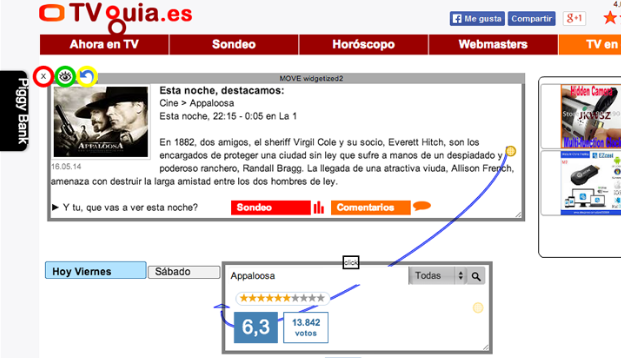
\includegraphics[width=0.5\textwidth]{figs/5-TVGuiaEditor.png}
	\label{fig:TVGuiaEditor}
}
\caption{Ejemplo de aumentación del sitio web de TVGuia.}
\label{fig:TVGuiaExample}
\end{figure}

\section{Validación}
\label{sec:ValidacionGenerador}

En este apartado, tomando como referencia los tres ejemplos que se han mostrado en el Apartado \ref{sec:EjemplosGenerador} se hace una validación de si las pruebas realizadas cubren todos los aspectos que hay que tener en cuenta, y garantizar si el generador realiza bien su trabajo.

Para ello hay que identificar los seis patrones posibles basados en blinks (Apartado \ref{sec:PatronesBlinks}) y los tres tipos de widgets (\textbf{HostBased}, \textbf{Cloned} y \textbf{ComplexCloned}).
\begin{itemize}
\item{HostBased: son los widgets propios de la página web.}
\item{Cloned: son elementos que se extraen de otros sitios webs.}
\item{ComplexCloned: son elementos extraídos de otros sitios webs donde su contenido es complejo. Los ComplexCloned tienen como objetivo, tomando algún elemento del sitio web variable, obtener cierta información remota. En el ejemplo de TVGuia, la película de la noche es variable (cada día hay una diferente). Mediante el buscador de un sitio remoto (en este caso filmaffinity) se puede obtener la puntuación de la película de la noche.}
\end{itemize}

Teniendo en cuenta estos aspectos, en la Tabla \ref{tab:ValidacionGenerador} se muestra qué tipos de widgets y qué patrones abarca cada uno de los ejemplos. Cómo se puede observar, entre los tres ejemplos se validan todos los patrones y los diferentes tipos de widgets, con lo que se puede asegurar que el generador cumple con sus funciones de manera adecuada.

\begin{table}
\centering
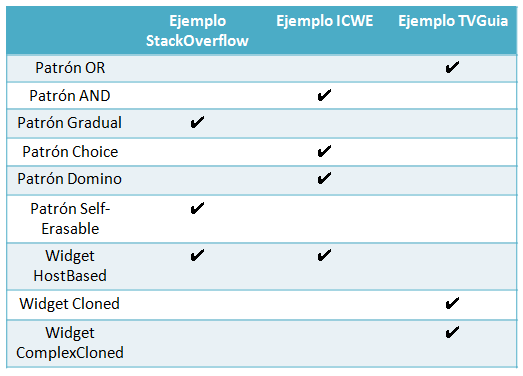
\includegraphics[width=0.7\linewidth]{./figs/5-Validacion.png}
\caption{Tabla de validación de los patrones y tipos de widgets basándose en los ejemplos.}
\label{tab:ValidacionGenerador}
\end{table} 